\documentclass[a4paper,11pt]{kth-mag}
\usepackage[T1]{fontenc}
\usepackage{textcomp}
\usepackage{lmodern}
\usepackage[utf8]{inputenc}
\usepackage[swedish, english]{babel}
\usepackage{modifications}
\usepackage{hyperref}
\usepackage{listings}
\usepackage{graphicx}
\usepackage{caption}
\usepackage{color}
\definecolor{gray}{rgb}{0.4,0.4,0.4}
\definecolor{darkblue}{rgb}{0.0,0.0,0.6}
\definecolor{cyan}{rgb}{0.0,0.6,0.6}


\lstset{
  basicstyle=\ttfamily,
  columns=fullflexible,
  showstringspaces=false,
  commentstyle=\color{gray}\upshape,
  captionpos=b
}

\lstdefinelanguage{XML}
{
  morestring=[b]",
  morestring=[s]{>}{<},
  morecomment=[s]{<?}{?>},
  stringstyle=\color{black},
  identifierstyle=\color{darkblue},
  keywordstyle=\color{cyan},
  morekeywords={xmlns,version,type}% list your attributes here
}

\title{Semantic parsing of Swedish laws}

\subtitle{Using RDF Lorem ipsum dolor sit amet, sed diam nonummy nibh eui
              mod tincidunt ut laoreet dol}
\foreigntitle{Lorem ipsum dolor sit amet, sed diam nonummy nibh eui
              mod tincidunt ut laoreet dol}
\author{Mikael Falgard}
\date{\today}
\blurb{Master's Thesis at NADA\\Supervisor: Sten Andersson\\Examiner: Anders Lansner}
\trita{TRITA xxx yyyy-nn}
\begin{document}
\frontmatter
\pagestyle{empty}
\removepagenumbers
\maketitle
\selectlanguage{english}
\begin{abstract}
  This is a skeleton for KTH theses. More documentation
  regarding the KTH thesis class file can be found in
  the package documentation.

Lorem ipsum dolor sit amet, consectetuer adipiscing elit. Mauris
purus. Fusce tempor. Nulla facilisi. Sed at turpis. Phasellus eu
ipsum. Nam porttitor laoreet nulla. Phasellus massa massa, auctor
rutrum, vehicula ut, porttitor a, massa. Pellentesque fringilla. Duis
nibh risus, venenatis ac, tempor sed, vestibulum at, tellus. Class
aptent taciti sociosqu ad litora torquent per conubia nostra, per
inceptos hymenaeos.
\end{abstract}
\clearpage
\begin{foreignabstract}{swedish}
  Denna fil ger ett avhandlingsskelett.
  Mer information om \LaTeX-mallen finns i
  dokumentationen till paketet. ÅÄÖ lalal

Lorem ipsum dolor sit amet, consectetuer adipiscing elit. Mauris
purus. Fusce tempor. Nulla facilisi. Sed at turpis. Phasellus eu
ipsum. Nam porttitor laoreet nulla. Phasellus massa massa, auctor
rutrum, vehicula ut, porttitor a, massa. Pellentesque fringilla. Duis
nibh risus, venenatis ac, tempor sed, vestibulum at, tellus. Class
aptent taciti sociosqu ad litora torquent per conubia nostra, per
inceptos hymenaeos.
\end{foreignabstract}
\clearpage
\tableofcontents*
\mainmatter
\pagestyle{newchap}

\part{Introduction}
\chapter{Introduction}

\section{Legal information online}

According to \textit{Rättsinformationsförordningen} (1999:175) basic legal information has to be provided both the public administration, and to private individuals in electronic form. For example the collection of statutory law, the \textit{Svensk Författningssamling} (SFS) is published in the Government Offices legal databases. These databases are old and hard to navigate since they only consist of plain text documents.

\section{Uniform standards}
One of the goals with \textit{Rättsinformationsförordningen} is that all legal information should be coherent, 
searchable from a single location and have a uniform presentation. Today’s decentralized system where 
authorities are responsible for their own documents, leads to a couple of problems. One of them being that 
the documents don’t follow the same format standards.\\\\ 
In 2006 a project called \textit{Rättsinformationsprojektet} was commenced to develop the legal information system further. 
A first step was to assure that the document that is going to be published contains the required meta data 
for that type of document. The next step is to assure that the information is delivered in a correct format.\footnote{Guidelines for publisher, developers etc are found on \url{http://www.lagrummet.se}} For example, date data must be unambiguously expressed in machine-readable form. 

\section{Rättsnätet} Rättsnätet is a free web service on
\url{www.notisum.se}\footnote{Notisum AB is the company that I am writing this thesis at.} that provides legal
information. Rättsnätet’s content consists of information gathered from
authority databases and is processed in several steps from pure text information
into a rich XML file. Notisum also provides a premium service that includes
additional information and services.

\section{Lagen.nu}
A similar website to Notisum is lagen.nu, they also provide all Swedish laws as a free web service. A difference is that lagen.nu follows standards regarding the Semantic Web\footnote{The Semantic Web is a collaborative movement that promotes common data formats on the World Wide Web.} in a better way than Notisum's Rättsnätet does. Lagen.nu is created by an individual with voluntary interest in law, the Semantic Web and is also involved in \textit{rättsinformationsprojektet}. 

\section{Problem}
Today Rättsnätet use processing steps that downloads, analyzes and transforms authority information from plain text to structured and marked up XML information. This process is a collection of programs written in Delphi Pascal and C\#. These programs, especially those that have been written in Delphi Pascal, are old and difficult to maintain. The conversion parts are constructed using a traditional technique similar to that used to write compilers.\\\\
Instead of using compiler technology lagen.nu use regular expressions to parse legal documents. The conversion programs lagen.nu use are written in object-oriented Python, which is more suitable for the task than Delphi Pascal that Notisum use today. Additionally lagen.nu is based on a document model from the Semantic Web, with the Resource Description Framework, RDF, as a base. Because of this the code base in lagen.nu has greater flexibility and is more about standards than Notisum.\\\\
The problem that this thesis focus on is how to modernize and replace Rättsnätet's current platform to a more modern process. A process where the result should be based on the Semantic Web and follow standards proposed by Rättsinformationsprojektet. Some aspects of the problem to keep in mind are:
\begin{itemize} 
\item The amount of documents, since there is over 200.000 legal documents, the program requires a fast process.
\item Legal source texts contains references that should be interpreted differently depending on the context, and to be marked up automatically with a certain margin of error.
\item Cross-references between the 200,000+ documents require theoretically, an array of 40 billion nodes.
\item The output from the process needs to be structurally similar to Notisums current process output so the post process (generating html) can be used with as little tweaking as possible.
\end{itemize}

\section{Limitations}
The implementation part of the thesis will be limited to the parsing step of the process. It will not cover the downloading or final transformation to html that is ready to be published.\\
To make this project feasible it is limited to handling only SFS data. Other types of data sources that a complete process would need to handle are for example: 
\begin{itemize}
\item Propositions
\item Supreme Court summaries
\item Decisions of the Courts of Appeal, and the Labour Court 
\item European legal regulations and directives
\end{itemize}
The goal is of course to create a generic and loosely coupled code base, so that it is easy to implement these 
modules in a later stage. 

\section{Abbreviations and Vocabulary} To be able to understand this report,
the reader needs to understand the following abbreviations. Given the
complexity of a legal document\footnote{For example "a paragraph" in a Swedish
legal document does not correspond to a regular paragraph in the English
language.} I will also present a vocabulary of how words are defined in the
thesis.

\subsection*{SFS} The Swedish Code of Statutes “Svensk författningssamling”
(SFS) is the official publication of all Swedish laws enacted by the Riksdag
and ordinances issued by the Government\footnote{SFS -
\url{http://en.wikipedia.org/wiki/Swedish_Code_of_Statutes}}. Every law and
ordinance has an SFS number, it consists of a four digit year, a colon, and
then an incrementing number by year. For instance the Ordinance on tattooing
dyes have the SFS number 2012:503\footnote{PDF copy of 2012:503 -
\url{http://notisum.se/rnp/sls/sfs/20120503.pdf}}.

\subsection*{SFSR}
The Statute Register (SFSR) includes registry information of Swedish Code
of Statutes (SFS), amendments, references to preparatory work, etc.

\subsection*{SFST}
Statutes in full text (SFST) includes Swedish Code of Statutes (SFS) in
full text, ie all applicable laws and regulations.

\subsection*{URI} Short for Unified Resource Identifier. Uniquely identifies
resources in a collection\footnote{URI - \url{http://www.w3.org/TR/uri-
clarification/}}, for example an hypertext transfer protocol url specifies a
webpage on the internet.

\subsection*{XML} Extensible Markup Language (XML) defines a set of rules for
encoding documents in a format that is readable for both humans and
machines\footnote{XML - \url{http://en.wikipedia.org/wiki/XML}}.

\subsection*{HTML} Hypertext Markup Language (HTML) is the main language for
displaying web pages and other information that can be displayed in a web
browser\footnote{HTML - \url{http://en.wikipedia.org/wiki/Html}}.

\subsection*{RDF} Resource Description Framwork (RDF) is a general method to
describe or model information that is implemented in web
resources\footnote{More detailed information about RDF in the ‘Background’
section}.

\subsection*{UTF-8} A encoding that can represent every character in the
Unicode character set. UTF-8 has become the dominant character encoding for
the World-Wide Web.

\subsection*{ISO-8859-1} A character encoding that is generally intended for
"Western European" languages, it encodes what it refers to as "Latin alphabet
no 1" consisting of 191 characters from the Latin script.

\subsection*{N3}
Notation3, or N3 is a shorthand non-XML serialization of RDF models,
designed with human-readability in mind which makes it more compact and
readable than XML RDF notation.

\subsection*{Dublin Core}
The Dublin Core metadata terms are a set of vocabulary terms which
can be used for simple resource description, or combining metadata
vocabularies of different metadata standards in Semantic web implementations.

\subsection*{The Semantic Web}
The word semantic stands for "the meaning of". The semantic of something is the meaning of something. The Semantic Web = a Web with a meaning.

\chapter{Background}

Lorem ipsum dolor sit amet, consectetuer adipiscing elit. Mauris
purus. 

\section{Swedish law}
The main legislative powers are the parliament (Riksdagen) and the government (Regeringen), these institutions can adopt statutes which are published in the main official collection of statutory law, the \textit{Svensk Författningssamling} (SFS). The statutes enacted by the parliament are referred to as laws, and the statutes enacted by the government as ordinances.\\\\
When a statute is changed, this is done by adopting a new statute (the change statute) that states what sections of the old statute (the base statute) are to be changed, and how. There is not a new merged version published of the statute in SFS, only the base statute and change statute(s).\\\\
Two recurring definitions in this paper are legal sources and legal source documents. A legal source is a type of legal information such as a constitution in SFS or verdicts from one of the Swedish courts. A legal source document is a specific document for a certain legal source, such as \textit{Personuppgiftslagen} (SFS 1998:204). 
\subsection{Law structure}
3000 gällande författningar, ingen exakt definerad struktur, kan se olika ut. 
Each law has an SFS number, including legislations amending already existing laws. The SFS number consists of a four digit year, a colon and a serial number assigned in chronological order of the date of issue. 

\subsection{Rättsinformationssystemet}
Rättsinformationssystemet is the state's system to make legal information such as laws, legislative histories, court cases, etc. - available to the public via the Internet. This information is produced by a number of different authorities. Today, each agency is responsible for publishing "their" information via their own website. It is all tied together by the website \url{http://www.lagrummet.se} which is referring to each agency's respective legal information page.\\\\
This decentralized approach has its advantages. It gives the authorities a lot of freedom to design their information in a way that fits them. A downside is that they use this freedom to invent their own standards. \textit{Rättsinformationsförordningen}\footnote{Rättsinformationssystemet is regulated in this ordinance (1999:175)} is not very detailed on how the information should be presented, only that it should be published.\\\\
An additional purpose with the system is the ability for the private sector to re-use government information to create added value services\footnote{Services like Rättsnätet from Notisum and lagen.nu}. Legal information is of great value, that could be even better utilized if it was easier to re-use the information.

\section{The Semantic Web - A Web with a meaning} 
The Semantic Web is a collaborative movement led by W3C\footnote{The international standards body, the World Wide Web Consortium (W3C} that promotes common data formats on the world wide web by encouraging semantic content in web pages. W3C's "Semantic Web Vision" is a future where: 
\begin{itemize}
\item Web information has exact meaning
\item Web information can be understood and processed by computers
\item Computers can integrate information from the web 
\end{itemize}

Natural languages have ambiguous meanings and even
a human reader may in some cases have problems understanding the correct
meaning of a text. If someone ask me  "Do you know Zlatan?" they may refer to if I know him as a friend or if Iknow who he is. It is the same for computers when they are trying to understand the meaning of a text. By adding labels to the text we can make it easier to interpret and thus creating a semantic web, formed so that software can collect and analyze data. The aim is that system can present the answer to a query instead of a page where the answer can be found, and answer queries where the answer is spread over several documents.
The semantic web is a web of data, where the data can be stored in documents in various ways. Using RDF is a way to structure data, so that it can be linked to other data with information and realations to objects.

\subsection{RDF}
Resource Description Framwork (RDF) is a general method to describe or model information that is implemented in web resources. It is based upon the idea of making statements about resources in the form of triples of subject-predicate-object. The subject denotes the resource (it can be anything that can have a URI), the predicate denotes traits or aspects of the resource and also expresses a relationship between the subject and the object. For example: "The sky" (subject) "has the color" (predicate) "blue" (object) could be an RDF triple.\\\\
Let's take a look at an example\footnote{Full example can be viewed at \url{http://www.w3schools.com/rdf/rdf_example.asp}} of an RDF object describing two CDs.
\begin{lstlisting}[language=xml, caption=An RDF example describing two records, label=rdfexample]
<?xml version="1.0"?>
<rdf:RDF 
  xmlns:rdf="http://www.w3.org/1999/02/22-rdf-syntax-ns#"
  xmlns:cd="http://www.recshop.fake/cd#">

  <rdf:Description
  rdf:about="http://www.recshop.fake/cd/Empire Burlesque">
    <cd:artist>Bob Dylan</cd:artist>
    <cd:country>USA</cd:country>
    <cd:company>Columbia</cd:company>
    <cd:price>10.90</cd:price>
    <cd:year>1985</cd:year>
  </rdf:Description>

  <rdf:Description
  rdf:about="http://www.recshop.fake/cd/Hide your heart">
    <cd:artist>Bonnie Tyler</cd:artist>
    <cd:country>UK</cd:country>
    <cd:company>CBS Records</cd:company>
    <cd:price>9.90</cd:price>
    <cd:year>1988</cd:year>
  </rdf:Description>
</rdf:RDF>
\end{lstlisting}
The lines \textbf{xmlns:rdf} and \textbf{xmlns:cd} define from which namespace elements with the rdf and cd prefix are from. The \textbf{rdf:Description} element contains the description of the resource identified by the \textbf{rdf:about} attribute. Finally the elements \textbf{cd:artist, cd:country, cd:company} etc. are properties of the resource.

\subsection{Other areas of use}
\subsubsection{Linked Data}
  
\chapter{Method}

The work with this thesis can be divided into two parts, the first being reading litterature regarding the Semantic Web and related subjects. The "litterature" included reading many articels, blog post and watching podcasts,\footnote{TODO, links to references, podcasts etc.} that were great to get a better understaning of the concept and importance of a more semantic web.\\\\  
The second part was to create a prototyp. Before I started to work on that I looked at the existing system, and tried to get some understanding of what steps the process went through. At this point a I got a lot of guidence from Magnus at Notisum, the author of the existing code. He explained the necessary steps and why they are important for the end result. However I didn't spend to much time on the old code, since I needed to create something different (and take factors such as semantics into mind).\\ With no background or knowledge in law it can be quite hard to understand the structure of laws and references between them. That is something I picked up as work went along with the prototype, many times I had to stop and try to figure out what I tried to do and why. 

\section{Methodology}
I devloped the prototype in several iterations, a simplfied version of agile.\footnote{Agile ... TODO} The first step was to get the program to read downloaded documents and save them as a new file. After that was in place, I always had a running prototype that would go through all files in a specified folder and apply transformations to them before saving them with a new exstension. This way I could add new functionality and try it out right away. I tried to put general functions and helpers seperate from SFS-specific logic so that it is possible to reuse a lot of the code when other legal sources needs to be implemented.     

\section{Existing system}

Below follows a short description of the steps the process goes through today. The steps in blue bubbles (first and last) are written in C\# and could with minor modifications be used together with the prototype. The two steps in pink bubbles (second step which is split in two different parts and the third step) are programs written in Pascal and will be replaced by the prototype. Then there's a green bubble (fourth step) which also with some modifications, could be reused with the output from the prototype.   
\begin{center}
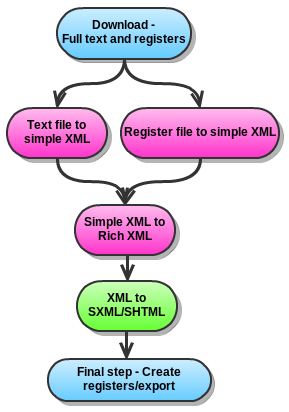
\includegraphics[scale=0.6]{imgs/oldSystemChart.png}
\captionof{figure}{Chart describing the existing process}
\end{center}
For the sake of simplicity lets say we are only handling SFS laws\footnote{In reality the program handles all kind of legal source documents.}. First we have a module that handles the actual downloading of the legal source files, (full text and register files\footnote{TODO, explain Registerfile} for each law) this part is written in C\# and could be reused\footnote{This part just have to download the files, then the prototype can do it's magic on those files.} for the prototype. Next we have two programs that for each law converts the downloaded files to very simple XML files, one for the full text and one for the registerfile. The next step is also an XML transformation, it takes the simple XML files and turns them into more comprehensive XML files. Now it's time to create files that can be viewed in a browser, this is done in several steps where data structures containing information regarding the laws are created with information like paragraph references and links. In the end a SHTML\footnote{TODO, explain SHTML} file that is ready to be published with this information is created. The final step is to export these files (and other legal source documents) to databases and update the website to display the newly created or updated files. 

\section{Prototype}
The main differences between the old system and the prototype are: 
\begin{itemize}
\item Language, the prototype is written in Python\footnote{TODO, something about python} which is a object oriented\footnote{something about OO} languge that is well suited for tasks like this one. It is easy to divide the code into separate modules that handle different tasks. Furthermore it is convinient to work with (apply transformations etc.) objects such as whole documents, paragraphs. 
\item Follows standards proposed by Rättsinformationsprojektet for legal documents.   
\item RDF, TODO: Marked up with URI's to.. 
\end{itemize} 

\subsection{Delimitations}
The prototype does not have to handle the downloading of the legal source documents, these can be presumed exist on the computer running the prototype. \\The aim for the prototype is to deliver XML files, the final step where these files are transformed into HTML files is simple and needs to be controlled by Notisum. However this step is done by the prototype but might not be the way Notisum will do it, if they use the prototype.

\part{Results}

\chapter{Implementation}

In this chapter I will discuss how the implementation was done and describe some implementation ideas and some parts of the prototype.\\\\

\section{Interface}
In order to interact with the program, read status and error information some sort of user interface is needed. Most common is a graphic user interface\footnote{A graphic user interface is a human-computer interface i.e., a way for humans to interact with computers.} that for example uses icons and menus. However, this falls outside the scope of this project, which focuses on the core of the program rather than the user experience. Instead, a rudimentary command line interface\footnote{Command line interface (CLI), an interface which use only text and are accessed solely by a keyboard. For example via an terminal in Linux.} was implemented, where the user can specify arguments at the start of the program (which is done via a terminal). During the parse and transformation process status updates will be presented in the terminal, for example if something fails the user will be notified. Also when the program is done the user will receive information about what was processed and the outcome.\\\\
The main file is called Controller.py and to run the program from a terminal an argument specifying what the program should do is needed. The intresting arguments for this thesis are 'ParseAll' and 'GenerateAll' other possible arguments are 'DownloadAll' and possible candidates to implement would be only 'Parse' or 'Generate' followed by a specific source, for example 'Parse 1997:240'. Also one can specify what types of legal sources that should be run, (will be relevant when more sources than SFS are implemented.) default behavior is to run for all types. There's also two available flags to use, '-d' for debug mode and '-h' or '--help' for help instructions.    

\begin{lstlisting}[language=bash, caption=Command to run the program]
kungen@dell-desktop:~$ python Controller.py --help
Usage: pyhton Controller.py [-d | -h] [arg]
Available flags are: -d (debug), -h--help (help)
kungen@dell-desktop:~$ python Controller.py
No arguments given
Valid arguments are: DownloadAll, GenerateAll, ParseAll
kungen@dell-desktop:~$ python Controller.py ParseAll
\end{lstlisting}

\section{Main modules}

\subsection{Controller.py}
The controller handles validation of user input (arguments and flags) if everything is correct it fetches all available legal source types (in this case just SFS) and then run the command given as an argument, ex. ‘ParseAll’ for each type.

\subsection{Source.py}
This module is a blueprint of how modules inheriting from it needs to look like. It contains the base classes for Controller and Parser, these classes contains functions that child classes need to implement and functions that can be overridden. Example of general functions are: checking if a file is up-to-date, trimming filenames or returning the XML or XHTML name for a certain file.\\
However most of the code will be specific for each legal source type and be implemented in the child modules. To support a new type of legal source for example 'EG Rättsfall'\footnote{European.. TODO}, create an 'EG' module that inherits Source.Controller and Source.Parser.

\subsection{SFS.py}
This is the module for parsing SFS documents, it fetches a list of all the downloaded files\footnote{The path to the base directory is specified in a config file, then it appends a path like ‘/sfs/dl/sfsr/1997’ for example for all SFS full text documents from 1997} and pass their file names one by one to the parser function if these three requirements are met:
\begin{enumerate}
\item If we have the file parsed already and it is newer than the incoming raw file, don't parse it again.
\item Filter out documents that is not proper SFS documents. They will have a name like ‘N1992:31’
\item Skip parsing the documents that have been or will be revoked, they are marked as “The constitution is repealed / shall be repealed”\footnote{“Författningen är upphävd/skall upphävas”}
\end{enumerate}

TODO: More about the steps in SFS. 

\section{Helper modules}

The helper modules are used to simplify (mostly) for the Parser by defining native python types, text readers etc.  

\subsection{DataObjects.py}

Makes it possible to build an object model for each legal source document, by
creating simple data objects. These objects are base data types that inherit
from native python types such as unicode, list, dict. The data types have
added support for other properties that can be set when instantiated.

\subsection{Reference.py}

Parses plaintext and finds references to other legal source documents and
returns a list with Link-objects\footnote{A Link-object is a base data type
that inherits from 'Unicode Structure' in DataObjects.py, basically a unicode
string with a 'URI' property.}. Depending on with which properties it is
initialized, it can find different types of references (Other laws,
'Rättsfall', 'EG-lagstiftning' etc..).

\subsection{TextReader.py}

Lorem ipsum dolor sit amet, consectetuer adipiscing elit. Mauris
purus. 

\subsection{Util.py}

A few small help functions mostly related to checking and or renaming directories and files. 

\section{Unicode}

Lorem ipsum dolor sit amet, consectetuer adipiscing elit. Mauris
purus. 

\section{3rd party libraries}

Lorem ipsum dolor sit amet, consectetuer adipiscing elit. Mauris
purus. 

\section{Version control}

GitHub\footnote{GitHub is a web-based hosting service for software development
projects that use the Git revision control system. \url{http://github.com}} is
used for web hosting and revision control, the code used for this report is
open source and available to checkout from the link below. On the github page
there's also an issue tracker with the current open issues, bugs and some
enhancements.\\\\
Project: \url{https://github.com/Sup3rgnu/lawParse}\\
Checkout: \url{https://github.com/Sup3rgnu/lawParse.git}

\chapter{Analysis}

\section{RDF}

Lorem ipsum dolor sit amet, consectetuer adipiscing elit. Mauris
purus.

\section{Rättsinformationsprojektet standard}

Lorem ipsum dolor sit amet, consectetuer adipiscing elit. Mauris
purus.  

\section{Performance}

Lorem ipsum dolor sit amet, consectetuer adipiscing elit. Mauris
purus. 



\chapter{Conclusions and Discussions}

Lorem ipsum dolor sit amet, consectetuer adipiscing elit. Mauris
purus. 

\section{Results}

Lorem ipsum dolor sit amet, consectetuer adipiscing elit. Mauris
purus. 

\section{Future development}

Lorem ipsum dolor sit amet, consectetuer adipiscing elit. Mauris
purus. 

\subsection{RDF Database}

Lorem ipsum dolor sit amet, consectetuer adipiscing elit. Mauris
purus. 

\chapter*{Bibliography}

[1] Ted Talk video about Linked Data with Tim Berners-Lee \url{http://www.ted.com/talks/tim_berners_lee_on_the_next_web.html}


\appendix
\addappheadtotoc
\chapter{RDF}\label{appA}

\begin{figure}[ht]
\begin{center}
And here is a figure
\caption{\small{Several statements describing the same resource.}}\label{RDF_4}
\end{center}
\end{figure}

that we refer to here: \ref{RDF_4}
\end{document}
